\renewcommand{\chaptername}{Cap\'itulo}
\chapter{Metodolog\'ia}
\label{Metodologia}

El cap\'titulo \ref{Metodologia} se organiza como sigue: al inicio se presentan  los modelos empleados para el desarrollo del servicio web, despu\'es, se describe el \textit{an\'alisis de requerimientos} que determina las actividades clave. Posteriormente, en la etapa de \textit{dise\~{n}o} de explican los modelos de referencia y en la \textit{implementaci\'on} se trabajan con etapas. Finalmente, se presenta una herramienta de \textit{evaluaci\'on} para estimar la usabilidad del servicio y se enumeran las tareas de \textit{mantenimiento}.

\section{Modelo de desarrollo}

Para el desarrollo del servicio web se emplearon principalmente dos modelos en distintos momentos, como modelo base, se emplea el de cascada \cite{IngDeSW} para las etapas de an\'alisis de requerimientos y dise\~{n}o, para las etapas subsecuentes, se adapt\'o el modelo incremental como una etapa m\'as que consiste en la codificaci\'on de m\'odulos reducidos, pruebas r\'apidas de funcionamiento, realimentaci\'on, correcci\'on, liberaci\'on o escalamiento para llegar a la implementaci\'on; la etapa final es la de mantenimiento como muestra la Figura \ref{modeloDesarrolloSW}. La descripci\'on de este modelo de  desarrollo se presenta en las secciones posteriores. 

\begin{figure}[!ht]
	\centering
	\fbox{
	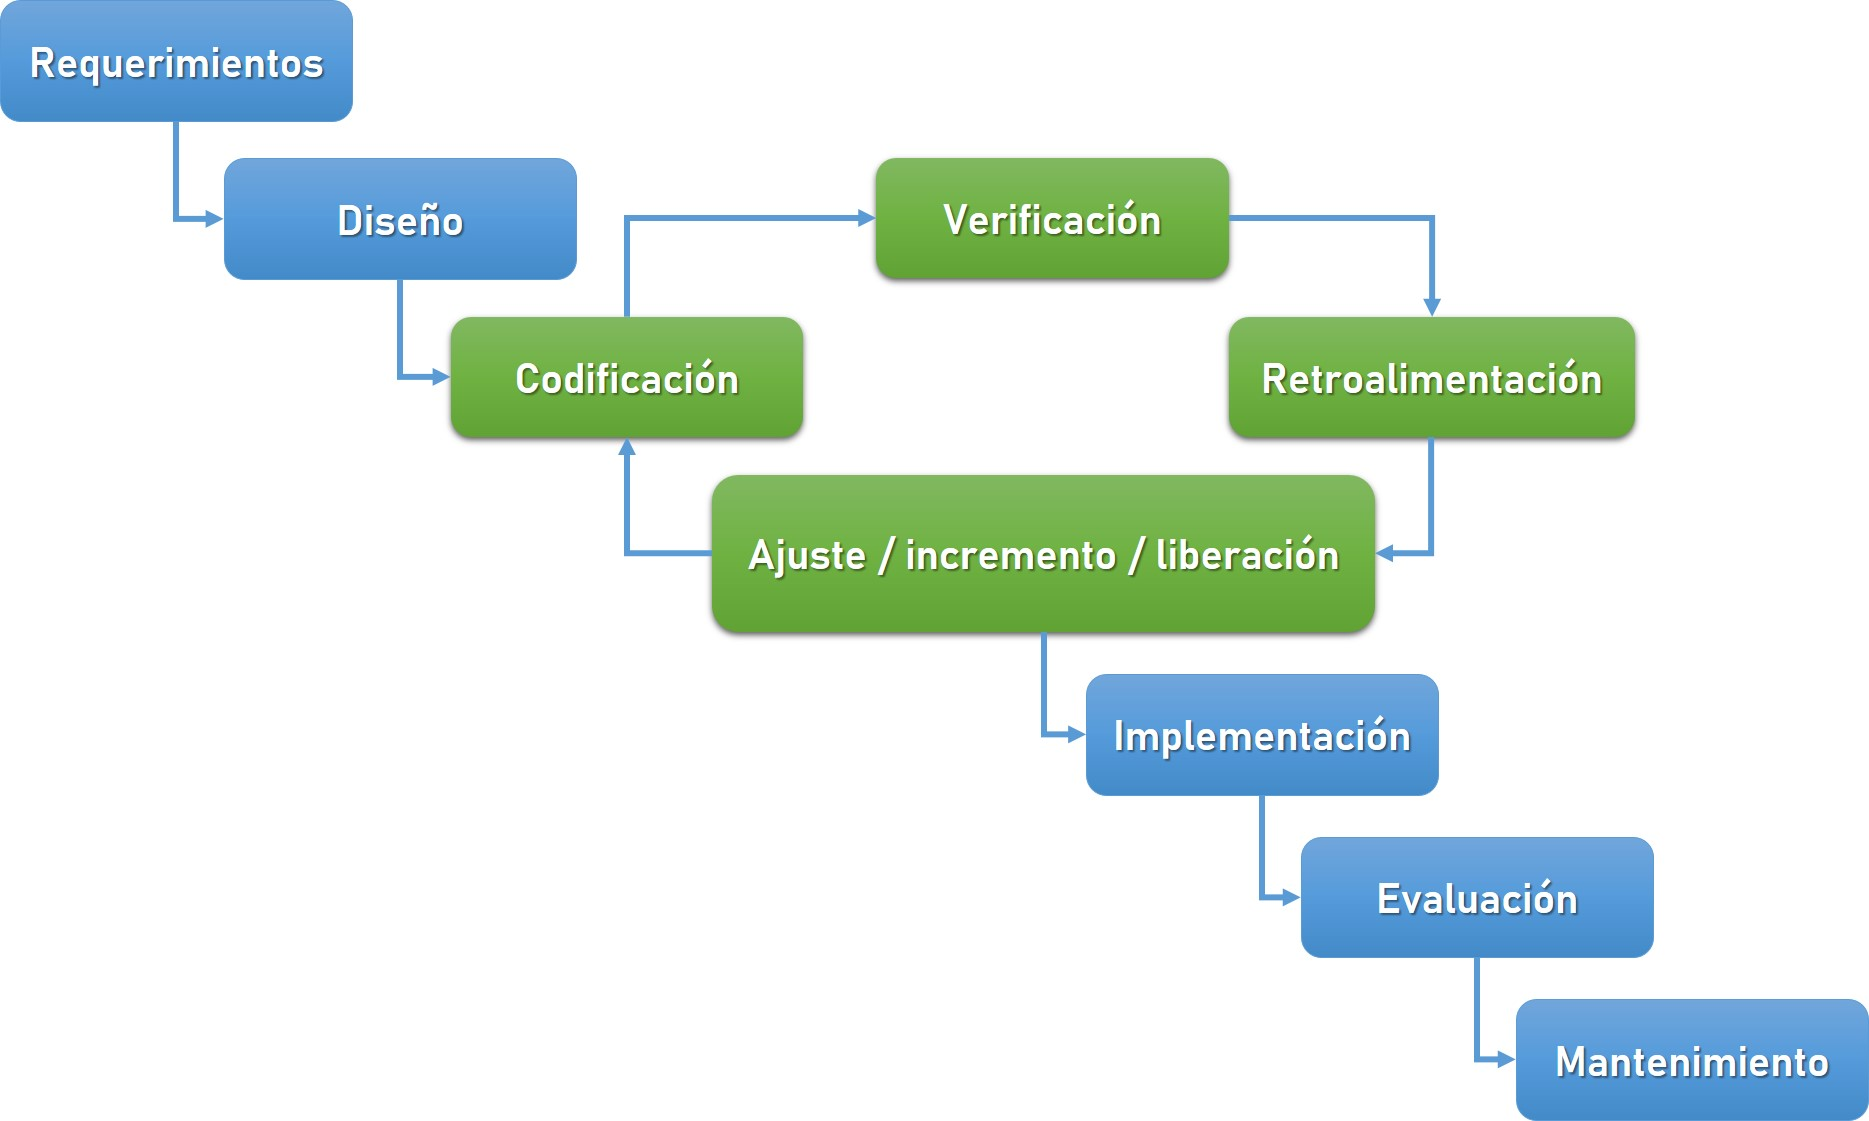
\includegraphics[width=12cm]{figures/ModeloDesarrolloSW.jpg}}
    \caption{Modelo de desarrollo del servicio web} %PIE DE LA IMAGEN
    \label{modeloDesarrolloSW}
\end{figure}

\section{An\'alisis de requerimientos}

El servicio web propuesto es parte del \emph{back end} del RI-UPPue,  el usuario final no tendr\'a una interacci\'on con \'este, sino que est\'a dise\~{n}ado para usuarios de tipo administrador. Junto con la administradora del RI-UPPue, se identificaron los requerimientos funcionales de la Tabla \ref{tablaRequerimientos}. 

\begin{table}[htbp]
    \begin{center}
    \caption{Tabla de requerimientos funcionales del servicio web}

    \begin{tabular}{|c|l|c|}
    \hline
    \centering \textbf{No. } & \textbf{Descripci\'on} & \textbf{Prioridad} \\
    \hline \hline
    1 & Consulta de informaci\'on sem\'antica & Alta  \\ \hline
    2 & Capacidad de almacenamiento de ternas en RDF & Alta  \\ \hline
    3 & Exportaci\'on de datos en formatos no propietarios como JSON y RDF & Mediana  \\ \hline
    4 & Integraci\'on de datos provenientes de otros RIs & Mediana  \\ \hline
    \end{tabular}
    \label{tablaRequerimientos}
    \end{center}
\end{table}

\section{Dise\~{n}o}

En la tesis se usan herramientas de modelado UML y los requerimientos planteados en la etapa de an\'alisis para elaborar los modelos de casos de uso, diagrama de clases y dise\~{n}o de alto nivel del servicio web, los cuales de describe a continuaci\'on.


\subsection{Casos de uso}

La Figura \ref{casoUso1} muestra el diagrama de casos de uso que modela la funcionalidad general del RI-UPPue.

\begin{figure}[!ht]
	\centering
	\fbox{
	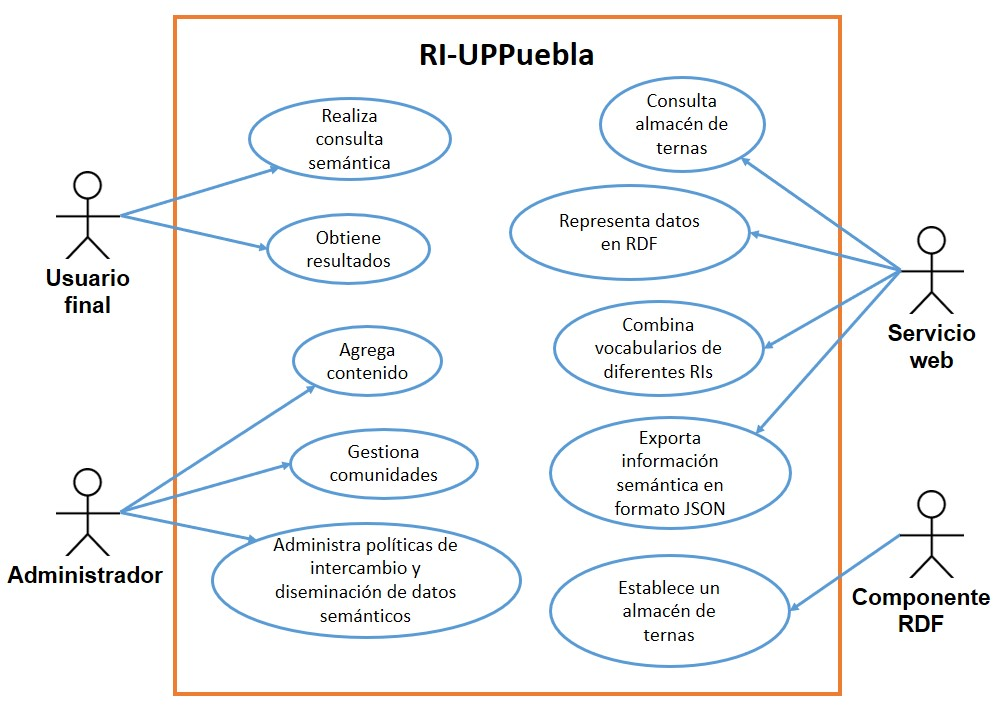
\includegraphics[width=12cm]{figures/CasoDeUso.jpg}} %NOMBRE DE LA FIGURA y TAMA\~{n}O
    \caption{Diagrama de casos de uso} %PIE DE LA IMAGEN
    \label{casoUso1}
\end{figure}

\subsection{Diagrama de clases}

La Figura \ref{diagramaClases1} muestra el diagrama de clases del servicio web, los rect\'angulos en color verde representan los nombres de las clases. Este dise\~{n}o se propuso en el art\'iculo \cite{SOMIdiseno}, en el cual se encuentra la descripci\'on detallada de los atributos y m\'etodos definidos para cada clase.

\begin{figure}[!ht]
	\centering
	\fbox{
	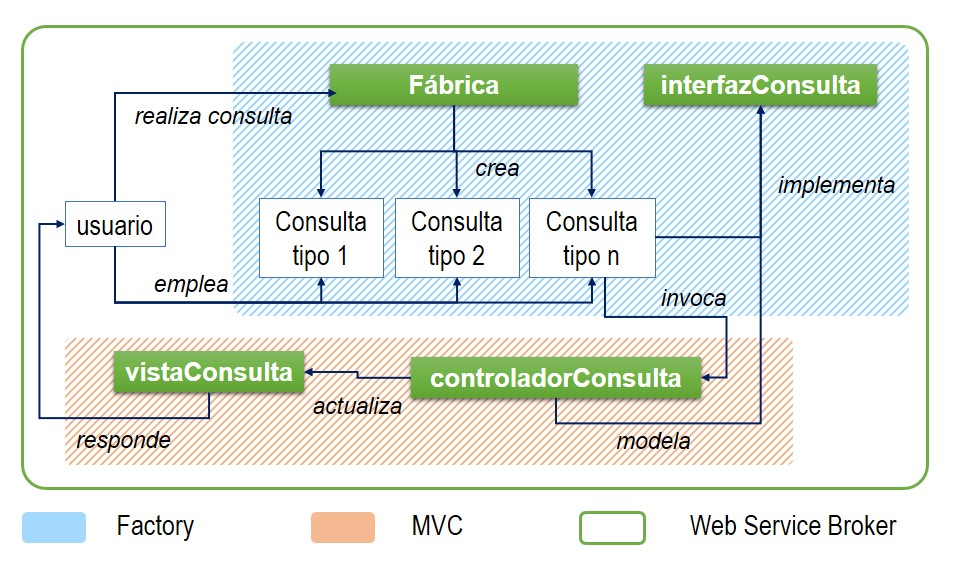
\includegraphics[width=12cm]{figures/Diagramadeclases1.jpg}} %NOMBRE DE LA FIGURA y TAMA\~{n}O
    \caption{Diagrama de clases. Fuente: \cite{SOMIdiseno}} %PIE DE LA IMAGEN
    \label{diagramaClases1}
\end{figure}

\subsection{Dise\~{n}o de alto nivel}

Las Figuras \ref{disenoAlto1} y \ref{disenoAlto2} muestran los dise\~{n}os elaborados para representar, por un lado, la manera en que se puede emplear el servicio web,  por otro lado, un modelo general del comportamiento en un contexto general, donde a corto plazo, se propone que opere en el  servidor del RI-UPPue y a mediano plazo, se buscar\'a su instalaci\'on en diferentes RIs que compartan la plataforma tecnol\'ogica DSpace.

\begin{figure}[!ht]
	\centering
	\fbox{
	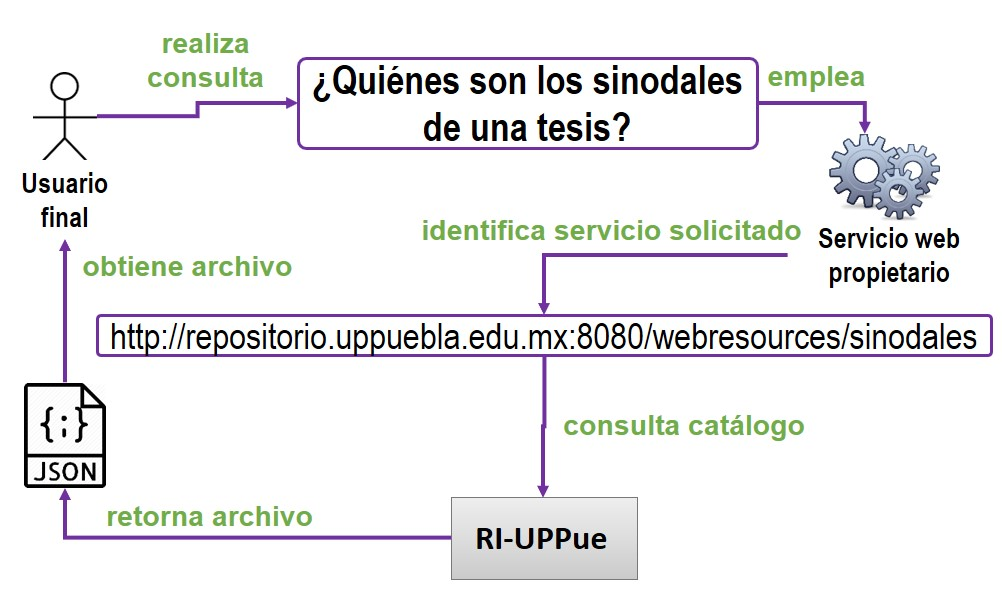
\includegraphics[width=12cm]{figures/DisenoAltoNivel1.jpg}} %NOMBRE DE LA FIGURA y TAMA\~{n}O
    \caption{Dise\~{n}o de consumo del servicio web. Fuente: \cite{SOMIdiseno}} %PIE DE LA IMAGEN
    \label{disenoAlto1}
\end{figure}

\begin{figure}[!ht]
	\centering
	\fbox{
	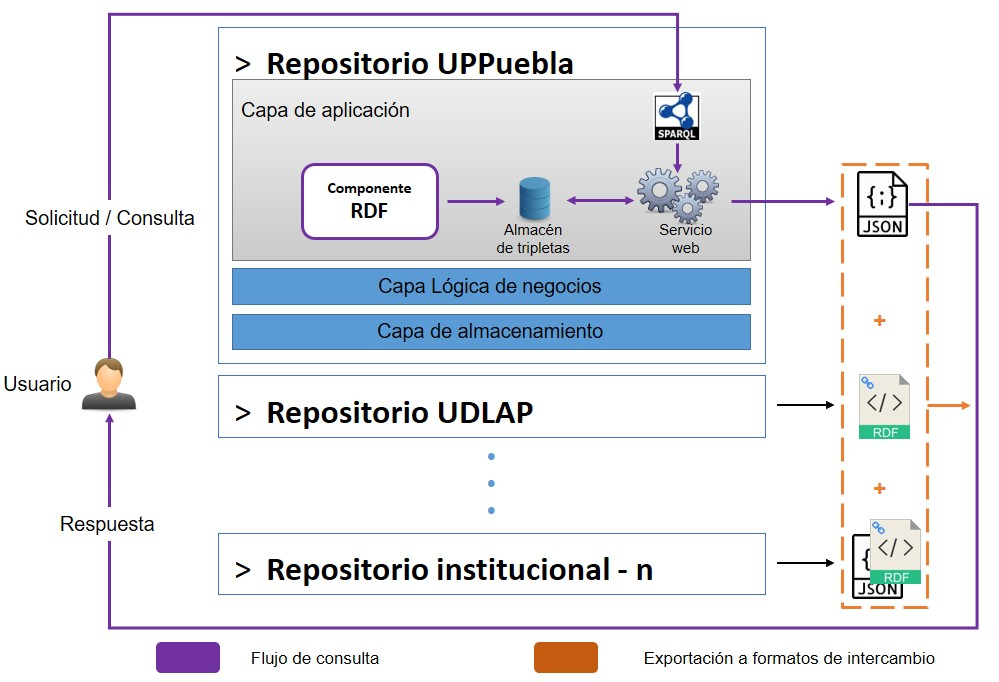
\includegraphics[width=12cm]{figures/DisenoAltoNivel2.jpg}} %NOMBRE DE LA FIGURA y TAMA\~{n}O
    \caption{Dise\~{n}o de alto nivel del servicio web. Fuente: \cite{SOMIdiseno}} %PIE DE LA IMAGEN
    \label{disenoAlto2}
\end{figure}

\section{Implementaci\'on}

Previo a la implementaci\'on de los m\'odulos, se asume que est\'a instalada la plataforma DSpace 6.2. Los pre-requisitos de operaci\'on para el servicio se relacionan con los elementos que muestra la Figura \ref{adicionalesDspace}, la cual contiene la arquitectura de la plataforma DSpace junto con los servicios adicionales que pueden ser habilitados. Cabe mencionar que la documentaci\'on de referencia de \cite{DSpaceRef} indica que DSpace cuenta con un m\'odulo RDF, sin embargo, \'este no se habilita durante la instalaci\'on est\'andar.

\begin{figure}[!ht]
	\centering
	\fbox{
	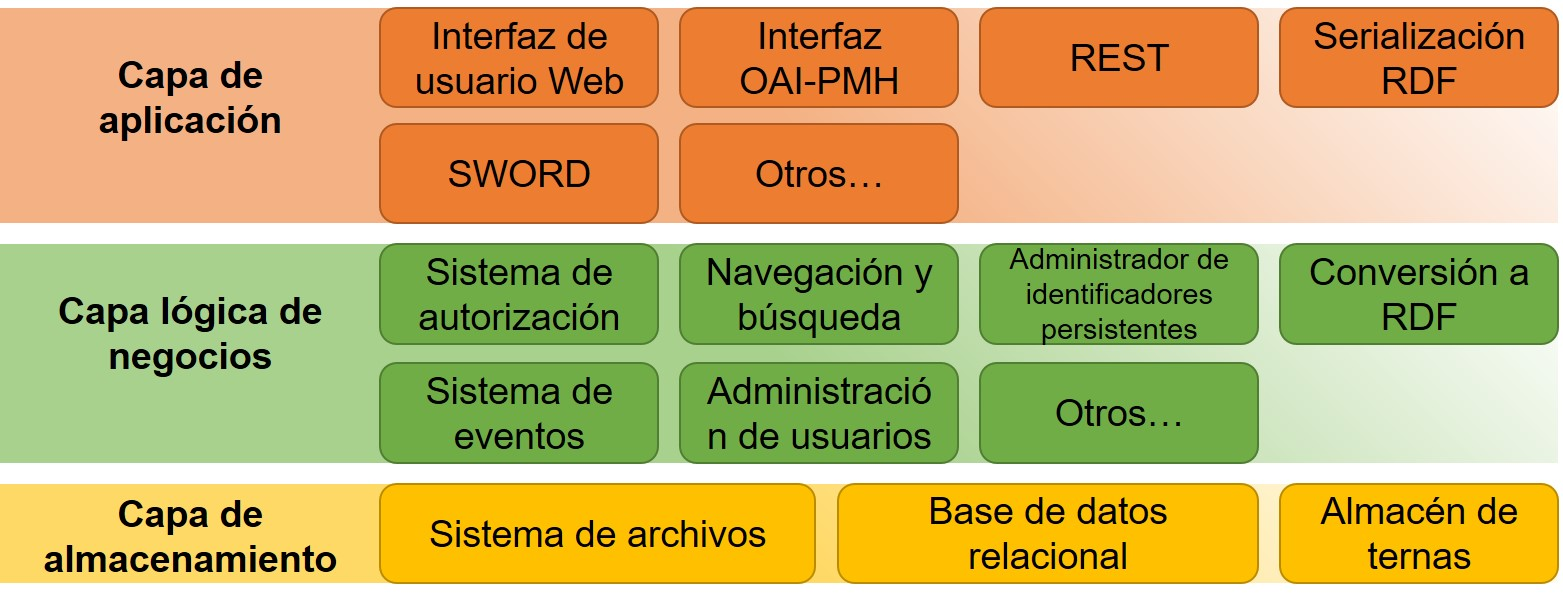
\includegraphics[width=12cm]{figures/ModulosAdicionalesDSpace62.jpg}} %NOMBRE DE LA FIGURA y TAMA\~{n}O
    \caption{M\'odulos adicionales de DSpace para la versi\'on 6.2} %PIE DE LA IMAGEN
    \label{adicionalesDspace}
\end{figure}

La habilitaci\'on del m\'odulo de serializaci\'on RDF requiere de tres elementos de software: 1) un almac\'en de ternas, 2) un mecanismo de serializaci\'on y 3) un conversor a formato RDF. La instalaci\'on de estos elementos forman parte de las etapas del proceso t\'ecnico que muestra la Figura \ref{etapasMigracion}, estas etapas se describen en las secciones siguientes.

\begin{figure}[!ht]
	\centering
	\fbox{
	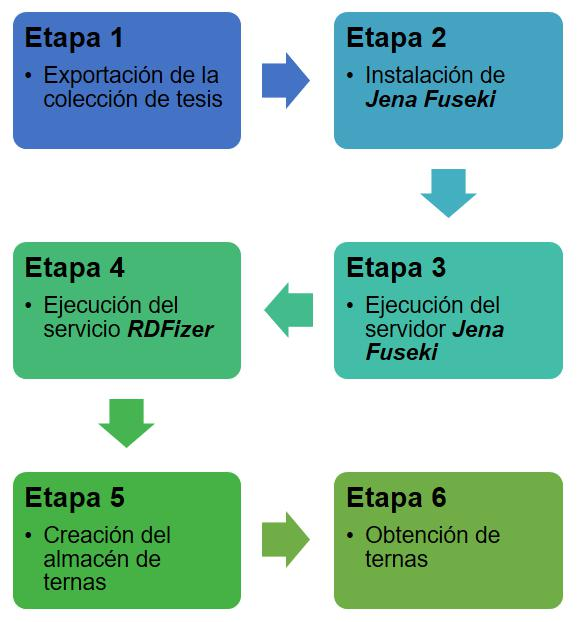
\includegraphics[width=10cm]{figures/etapasMigracion.jpg}} %NOMBRE DE LA FIGURA y TAMA\~{n}O
    \caption{Etapas del proceso de migraci\'on de metadatos del RI-UPPue a la web sem\'antica} %PIE DE LA IMAGEN
    \label{etapasMigracion}
\end{figure}

\subsection{Etapa 1: exportaci\'on de la colecci\'on de tesis}

DSpace permite exportar cualquier colecci\'on, en particular, se emplea la colecci\'on de tesis del RI-UPPue, formada por m\'as de  50 tesis del Departamento de Posgrado. La Figura \ref{exportacion-csv} muestra la interfaz para esta tarea, los metadatos se almacenan a un archivo con extensi\'on CSV\footnote{Siglas del ingl\'es de \emph{Comma Separated Values}, formato separado por comas}. El n\'umero 1 muestra el bot\'on para exportar y el 2 el archivo CSV con los metadatos exportados. La tarea de exportaci\'on se llev\'o a cabo al utilizar la versi\'on 75.0.3770.142 del navegador Chrome y la interfaz en JSP de DSpace.

\begin{figure}[!ht]
	\centering
	\fbox{
	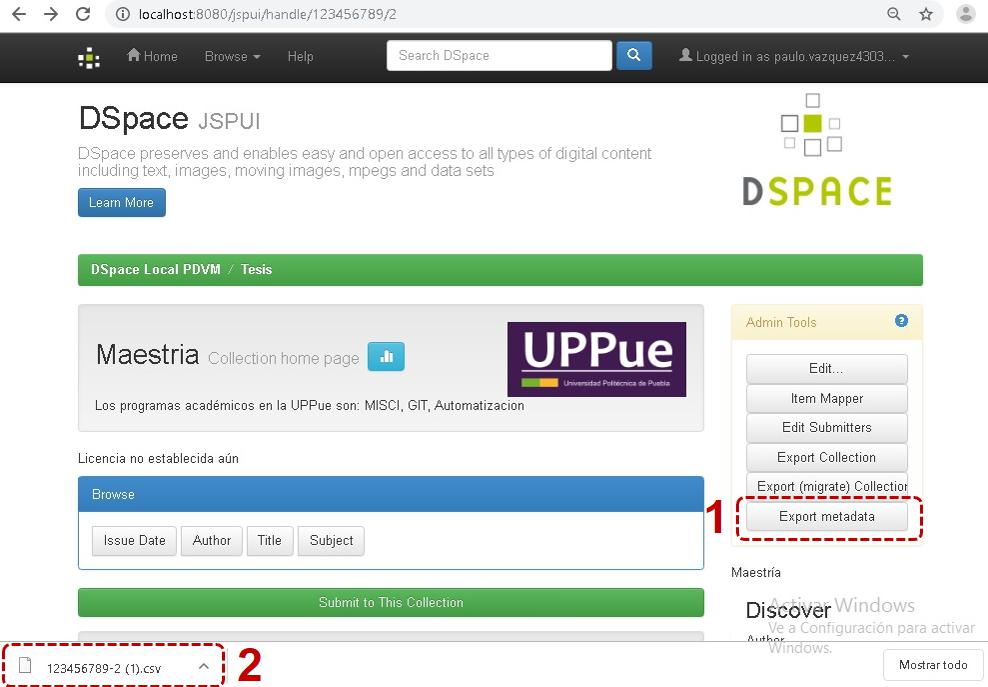
\includegraphics[width=12cm]{figures/exportarCSV.jpg}} 
    \caption{Exportaci\'on de la colecci\'on tesis a \textit{CSV}}
    \label{exportacion-csv}
\end{figure}

\subsection{Etapa 2: instalaci\'on de Apache Jena Fuseki}

El almac\'en de ternas es Jena-Fuseki versi\'on 1.6.0, este servidor provee tambi\'en de una interfaz web para realizar consultas en lenguaje SPARQL. Fuseki se integra con TDB\footnote{Componente de Jena Fuseki para el almacenamiento y consulta de datos en RDF} para proporcionar una capa de almacenamiento persistente transaccional y robusta, permite consultas de texto y consultas espaciales \cite{JenaFuseki}. La p\'agina oficial de Apache Jena Fuseki\footnote{Disponible en https://jena.apache.org/download/index.cgi} prove\'e diversas opciones para la descarga dependiendo del sistema operativo: Linux (.tar.gz) o Windows(.zip). 

\begin{figure}[!ht]
	\centering
	\fbox{
	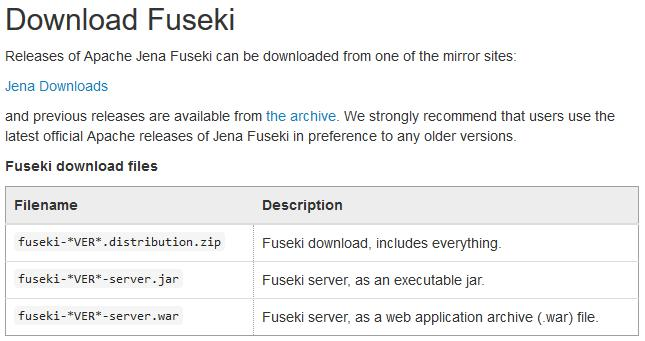
\includegraphics[width=12cm]{figures/opcionesDescargaFuseki.jpg}} 
    \caption{Opciones de descarga para el almac\'en de ternas Jena Fuseki}
\label{opcionesDescargaFuseki}
\end{figure}

Para terminar la instalaci\'on, los archivos descargados se descomprimen y se guardan en una carpeta que se nombra como \textit{Fuseki}. 

\begin{figure}[!ht]
	\centering
	\fbox{
	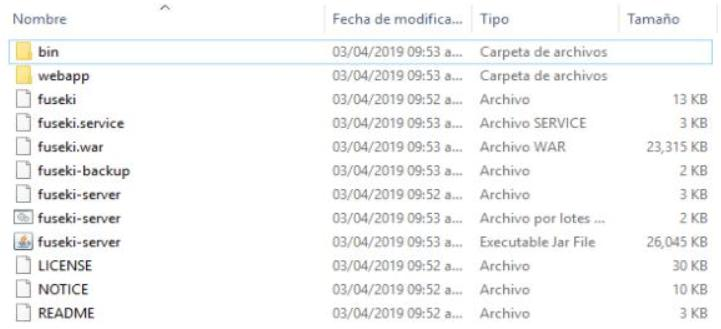
\includegraphics[width=12cm]{figures/contenidoCarpetaJena.jpg}} 
    \caption{Contenido de la carpeta del servidor \textit{Jena Fuseki}}
    \label{opcionesDescargaFuseki}
\end{figure}

\subsection{Etapa 3: ejecuci\'on del servidor Jena Fuseki}

Jena Fuseki se ejecuta como servicio de sistema operativo, como aplicaci\'on web Java (WAR) o como servidor independiente. El componente \texttt{Apache Shiro} se utiliza para implementar caracter\'isticas de seguridad, tiene una interfaz de usuario para el monitoreo y la administraci\'on. Jena Fuseki se inicializa ejecutando el archivo \textit{fuseki-server.bat}, (\textit{.jar} en Linux) como muestra la Figura \ref{ejecucionFuseki}.

\begin{figure}[!ht]
	\centering
	\fbox{
	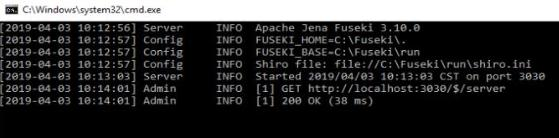
\includegraphics[width=12cm]{figures/ejecucionFuseki.jpg}} 
    \caption{Ejecuci\'on del servidor Jena Fuseki en terminal de Windows}
    \label{ejecucionFuseki}
\end{figure}

\subsection{Etapa 4: ejecuci\'on del servicio RDFizer}

Un componente \texttt{RDFizer} \cite{RDFizer} o \textit{spongers}, transforma datos de DSpace en una o m\'as de las serializaciones al modelo de datos RDF. La Figura \ref{etl-diagrama} representa esta transformaci\'on. Los \texttt{RDFizers} implementan  las tareas b\'asicas siguientes: extraer, transformar y cargar, en ingl\'es, \emph{extract}, \emph{transform} y \emph{load} (ETL), mismas que se describen como sigue: 

\begin{itemize}
    \item \textit{Extraer}. Los datos se obtienen de una base de datos o se recopilan de m\'ultiples y diversas fuentes 
    
    \item \textit{Transformar}. Los datos obtenidos se transforman en los requeridos mediante formularios; la transformaci\'on utiliza reglas o tablas de b\'usqueda o combina los datos con otros.
    
    \item \textit{Cargar}. Los datos se escriben en la fuente o base de datos destino. 
\end{itemize}

\begin{figure}[!ht]
	\centering
	\fbox{
	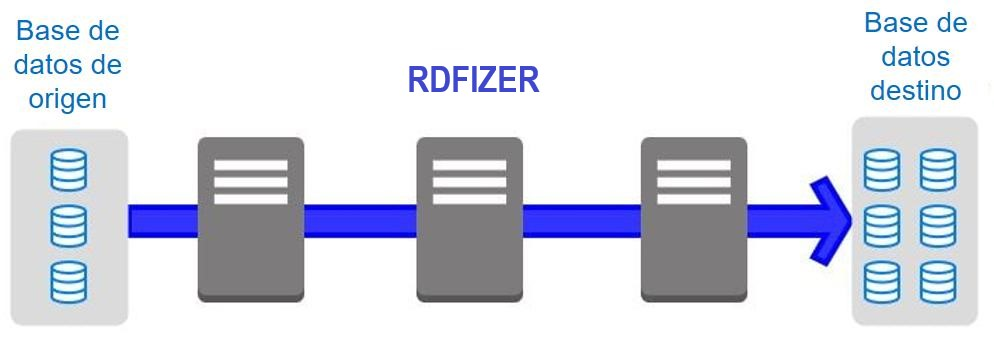
\includegraphics[width=12cm]{figures/etl.jpg}} 
    \caption{Extracci\'on, transformaci\'on y carga}
    \label{etl-diagrama}
\end{figure}

Los \texttt{RDFizers} soportan la migraci\'on de los metadatos a formatos de intercambio como XML, RDF o JSON. 

\subsection{Etapa 5: creaci\'on del almac\'en de ternas}

Una vez que los metadatos del repositorio se han procesado por los RDFizes o ETLs, los archivos con datos en RDF se almacenan en la ubicaci\'on indicada en el archivo de configuraci\'on de la plataforma DSpace \textit{fuseki-assembler-ttl}, forman as\'i el almac\'en de ternas o servicio persistente.

\subsection{Etapa 6: obtenci\'on de ternas}

Los metadatos en RDF para cada tesis se acceden empleando una direcci\'on de internet o URL\footnote{Localizador Uniforme de recursos, en ingl\'es \textit{Uniform Resource Locator}} como muestra la Figura \ref{accesoRdf}.\newline

\begin{figure}[!ht]
	\centering
	\fbox{
	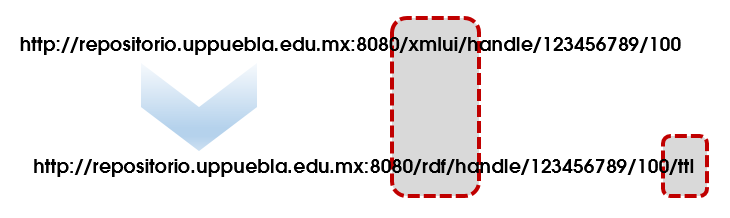
\includegraphics[width=12cm]{figures/xmluiRdf.png}} 
    \caption{Acceso a metadatos de tesis en RDF}
    \label{accesoRdf}
\end{figure}

La Figura \ref{resultadoRdf} muestra algunos metadatos de una tesis en RDF. Note que el archivo RDF contiene los metadatos capturados en la plataforma DSpace cuando se agrega un documento a la colecci\'on. En el ejemplo, se muestra un error l\'ogico, notar que los elementos \texttt{creator} y \texttt{contributor} contienen el mismo valor.

\begin{figure}[!ht]
	\centering
	\fbox{
	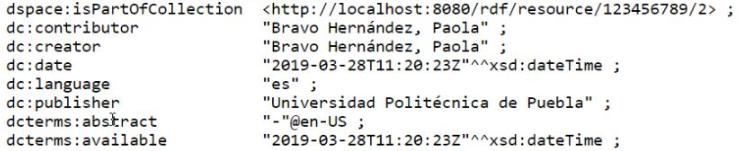
\includegraphics[width=12cm]{figures/extractoMetadatosRDF.jpg}} 
    \caption{Metadatos de RDF para una tesis del almac\'en de ternas}
    \label{resultadoRdf}
\end{figure}

\subsection{Interfaz gr\'afica de usuario}

La interfaz gr\'afica de usuario (\emph{Graphical User Interface}, GUI) o \emph{front end} del servicio web propuesto, integra tres tecnolog\'ias web: 
\emph{HTML 5}, lenguaje de modelado de hipertexto, en ingl\'es \emph{HiperText Markup Language}, que es un lenguaje de marcado que sirve para modelar contenidos; \emph{Java Script}, que es un lenguaje de programaci\'on del lado del cliente para manipular elementos HTML y hojas de estilo en cascada, en ingl\'es \emph{Cascading Style Sheets} (CSS), que sirven para definir reglas de dise\~{n}o para la presentaci\'on del contenido. Estas tecnolog\'ias son nativas a la web por lo que no se requiere de ning\'un tipo de instalaci\'on adicional, ya que ejecuci\'on de los modelos se realiza a trav\'es del uso navegadores como  Chrome, Mozilla, Opera, Edge o Safari.

\subsection{Herramientas software}

Esta secci\'on contiene una breve descripci\'on de las herramientas de software utilizadas en la implementaci\'on del servicio web. 

\subsubsection{Servicio especializado en lenguaje Python 3.6}

Se utiliz\'o la versi\'on 3.6 del lenguaje de programaci\'on Python para extraer elementos (\emph{\'items}) del almac\'en de ternas a trav\'es de la librer\'ia RDFLib  versi\'on 4.2.2  \cite{RDFlib} y as\'i integrar los datos provenientes del RI-UPPue a una instancia de la ontolog\'ia Onto4-RI-UPPue a trav\'es de la librer\'ia OWLReady2 \cite{OWLReady2} versi\'on 0.19. La Figura \ref{arquitecturaServicio} muestra la arquitectura propuesta para el servicio web y sus componentes. 

\begin{figure}[!ht]
	\centering
	\fbox{
	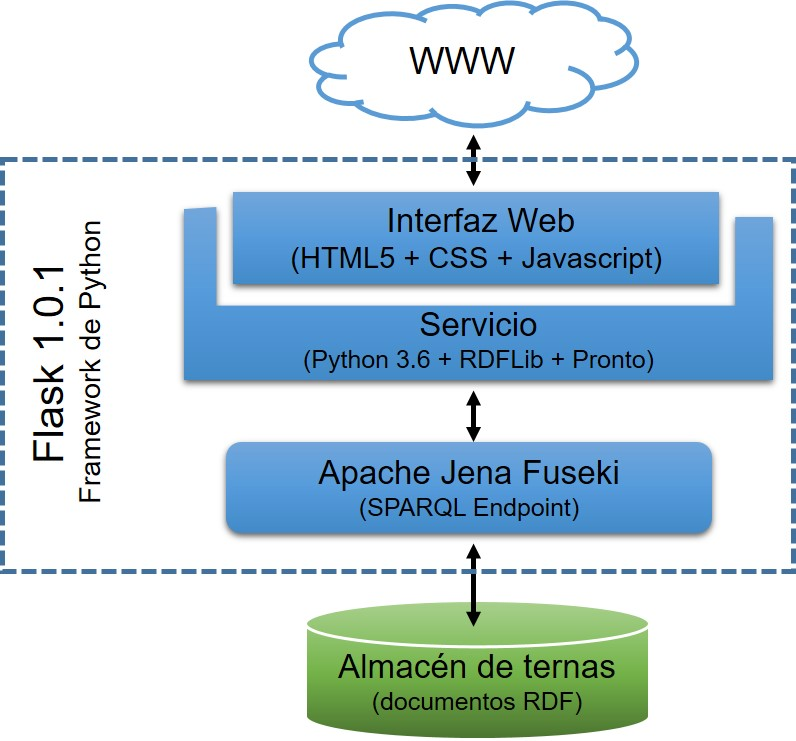
\includegraphics[width=10cm]{figures/ArquitecturaSW.jpg}} 
    \caption{Arquitectura del servicio web}
    \label{arquitecturaServicio}
\end{figure}

La Figura \ref{tecnologiasServicio} muestra las tecnolog\'ias empleadas para el desarrollo del servicio web desde el punto de vista del \emph{front end} (parte gr\'afica del servicio web) y del \emph{back end} (parte l\'ogica del servicio web).

\begin{figure}[!ht]
	\centering
	\fbox{
	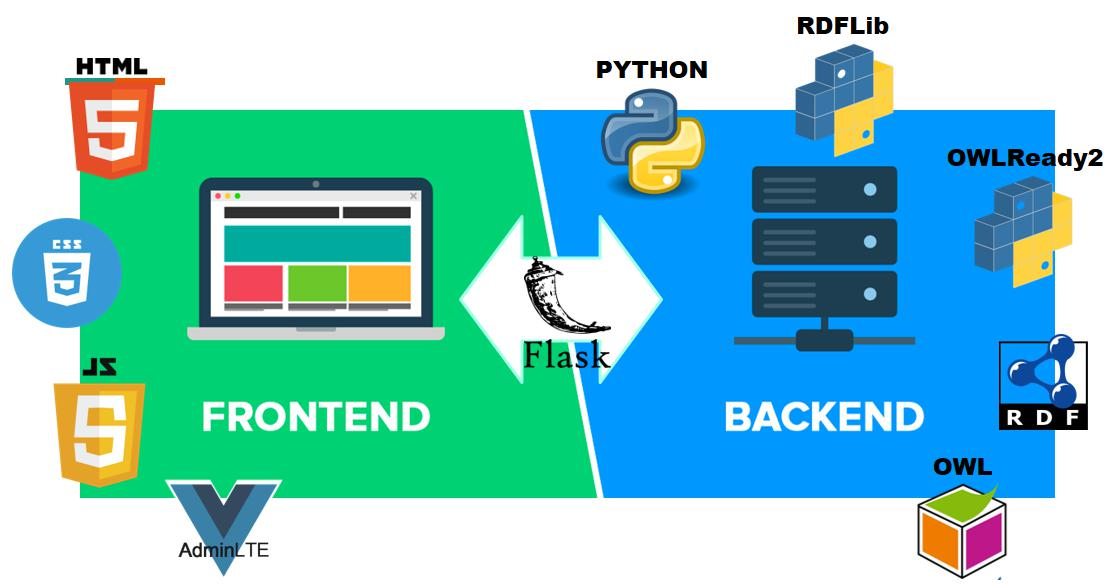
\includegraphics[width=12cm]{figures/tecnologiasServicoWeb.jpg}} 
    \caption{Tecnolog\'ias empleadas en el servicio web}
    \label{tecnologiasServicio}
\end{figure}

\subsubsection{Librer\'ia RDFLib}

La librer\'ia \texttt{RDFLib}\footnote{Disponible en: \textit{https://pypi.org/project/rdflib/}} de Python sirve para trabajar con datos en RDFen diferentes sintaxis como \texttt{RDF/XML, N3, NTriples, Turtle, TriX, RDFa} y \texttt{Microdata}; su interfaz \textit{Graph} puede ser respaldada por cualquiera de las implementaciones de \textit{Store}. El n\'ucleo \texttt{rdflib} incluye implementaciones de \texttt{Store} para almacenamiento en memoria, almacenamiento persistente (en Berkeley DB) y un contenedor para puntos finales remotos de SPARQL, incluye el motor de consulta SPARQL 1.1.

La instalaci\'on de \texttt{RDFLib} se realiza a trav\'es del servicio \textit{pip}\footnote{Repositorio de software para el lenguaje Python, en ingl\'es \textit{Python Index Package} } de Python mediante la instrucci\'on \texttt{pip install rdflib} como se indica en la documentaci\'on de este lenguaje. 

\subsubsection{Librer\'ia OWLReady2}

La librer\'ia OWLReady2\footnote{Disponible en \emph{https://pypi.org/project/Owlready2/}}  de Python se usa trabajar con ontolog\'ias escritas en la versi\'on 2.0 de OWL, las cuales se gestionan como objetos Python. La librer\'ia soporta la conexi\'on el razonador Hermit y tareas como las siguientes: 

\begin{itemize}
    \item Importaci\'on de ontolog\'ias OWL 2.0 en NTriples, RDF/XML o formato OWL/XML.
    \item Exportaci\'on de ontolog\'ias OWL 2.0 a NTriples o RDF/XML
    \item Manipulaci\'on de clases, instancias y propiedades de las ontolog\'ias de forma transparente, como si fueran objetos de Python
    \item Agregaci\'on de m\'etodos de Python a las clases de una ontolog\'ia
    \item Clasificaci\'on autom\'atica de clases e instancias utilizando los razonadores HermiT o Pellet 
    \item Compatibilidad con la librer\'ia RDFlib 
  \end{itemize}

\subsubsection{Librer\'ia xml.etree.ElementTree}

La librer\'ia \textit{xml.etree.ElementTree}\footnote{Disponible en \textit{https://pypi.org/project/elementtree/}} se usa para procesar documentos XML, cuenta con diversos m\'etodos para acceder a elementos espec\'ificos de un documento, insertar, modificar y eliminar nodos. En la tesis, esta librer\'ia se utiliza para obtener informaci\'on de la ontolog\'ia Onto4RI-UPPue escrita en OWL.

\subsubsection{Framework Flask}

El desarrollo del servicio web emplea la versi\'on 1.1.1 de Flask \footnote{Disponible en \emph{https://pypi.org/project/Flask/}}, el cual es un \emph{framework} ligero para aplicaciones web, es decir, entorno de trabajo o marco de trabajo, conjunto estandarizado de conceptos, pr\'acticas y criterios para enfocar un tipo de problem\'atica particular que sirve como referencia para enfrentar y resolver nuevos problemas de \'indole similar. 

Flask est\'a dise\~{n}ado para desarrollar proyectos de manera r\'apida y relativamente sencilla con capacidad para escalar a aplicaciones complejas, implementa el patr\'on de dise\~{n}o Modelo-Vista-Controlador (MVC), en ingl\'es \emph{Model-View-Controller}, ampliamente usado en el desarrollo de proyectos de software. 

\subsubsection{AdminLTE}
Finalmente, en el desarrollo del \emph{front end} se integra el panel de control o \emph{Dashboard} que conforma un tipo de interfaz gr\'afica de usuario con\emph{AdminLTE},  versi\'on 2.4.15.

\section{Evaluaci\'on}

Las pruebas de usabilidad orientadas a la experiencia del usuario \footnote{Tambi\'en conocido como \emph{UX}, en ingl\'es \emph{User eXperience}} se basan en la observaci\'on y an\'alisis de un grupo de usuarios reales empleando el servicio web, con objeto de identificar los problemas de uso. El servicio web se eval\'ua a trav\'es de una adaptaci\'on de la plantilla para hacer an\'alisis heur\'isticos de usabilidad\footnote{Disponible en \emph{https://www.torresburriel.com/weblog/2008/11/28/plantilla-para-hacer-analisis-heuristicos-de-usabilidad/}} propuesta por \cite{OnceHeuristicas}. La herramienta consta de un cuestionario que explora once heur\'isticas y en donde el evaluador (en este caso, un usuario) indica seg\'un una escala de Likert de cinco grados, su grado de satisfacci\'on. La Tabla \ref{tablaEscalasLikert} muestra las escalas con las que se eval\'uan cada una de las heur\'isticas.\newline

\begin{table}[htbp]
    \begin{center}
    \caption{Escala de Likert empleada para evaluar el servicio web}
    \begin{tabular}{| p{1.5cm}| p{11cm} |}
    \hline
    \centering \textbf{Valor } & \textbf{Observaciones} \\
    \hline \hline
    1 & Se da la m\'inima expresi\'on del heur\'istico en las p\'aginas evaluadas \\ \hline
    2 & Se da una expresi\'on baja del heur\'istico en las p\'aginas evaluadas \\ \hline
    3 & Se da una expresi\'on media del heur\'istico en las p\'aginas evaluadas \\ \hline
    4 & Se da una expresi\'on alta del heur\'istico en las p\'aginas evaluadas \\ \hline
    5 & Se da la m\'axima expresi\'on del heur\'istico en las p\'aginas evaluadas \\ \hline
    \end{tabular}
    \label{tablaEscalasLikert}
    \end{center}
\end{table}

Las heur\'isticas evaluadas son las siguientes:

\begin{itemize}
    \item Generalidades
    \item Identidad e informaci\'on
    \item Lenguaje y redacci\'on
    \item Rotulado
    \item Estructura y navegaci\'on
    \item Estructura de la p\'agina
    \item B\'usqueda
    \item Elementos multimedia
    \item Ayuda
    \item Accesibilidad
    \item Control y retroalimentaci\'on
\end{itemize}

\begin{figure}[!ht]
	\centering
	\fbox{
	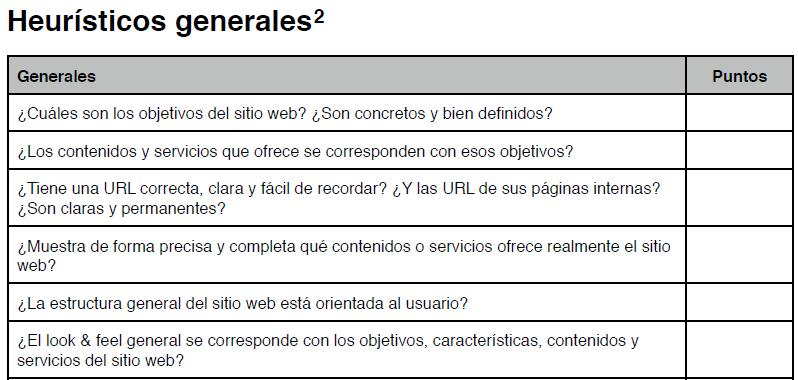
\includegraphics[width=12cm]{figures/extractoPlantilla.jpg}} 
    \caption{Extracto de la plantilla para hacer an\'alisis heur\'isticos de usabilidad}
    \label{extractoPlantilla}
\end{figure}

\section{Mantenimiento}

La fase final del desarrollo del servicio web consta de realizar las modificaciones o adecuaciones identificadas en la etapa de evaluaci\'on.
